\chapter{Implementierung}

% \section{Architektur}
% Um eine geeignete Architektur für die Realisierung der Bibliothek an Schwarmintelligenz-Algorithmen zu finden, wurden zunächst die einzelnen Algorithmen untersucht und versucht aus Gemeinsamkeiten Abstraktionen zu entwickeln.
% \subsection{BaseSwarm}
% Dazu wurde ein abstraktes Package mit dem Namen 'BaseSwarm' entwickelt, die ein Basisskelett für alle abzubildenden Algorithmen bildet. 
% Base Swarm unterteilt sich in die abstrakten Klassen (vgl. \autoref{uml_img}):
% \begin{itemize}
%     \item Swarm
%     \item SwarmGroup
%     \item SwarmMember
%     \item Swarm Solution
% \end{itemize}
% begleitet von den Interfaces:
% \begin{itemize}
%     \item IFunction
%     \item ISwarmMember
%     \item ISwarmSolve
%     \item ISwarmVisitor
% \end{itemize}
% Alle dargestellten Klassen des Packages sind abstrakt definiert, da von diesen für die Zielalgorithmen abgeleitet werden soll. 




\section{Design Patterns}
\subsection{Facade}
\subsection{Visitor}

\begin{figure}[ht]
    \begin{center}
        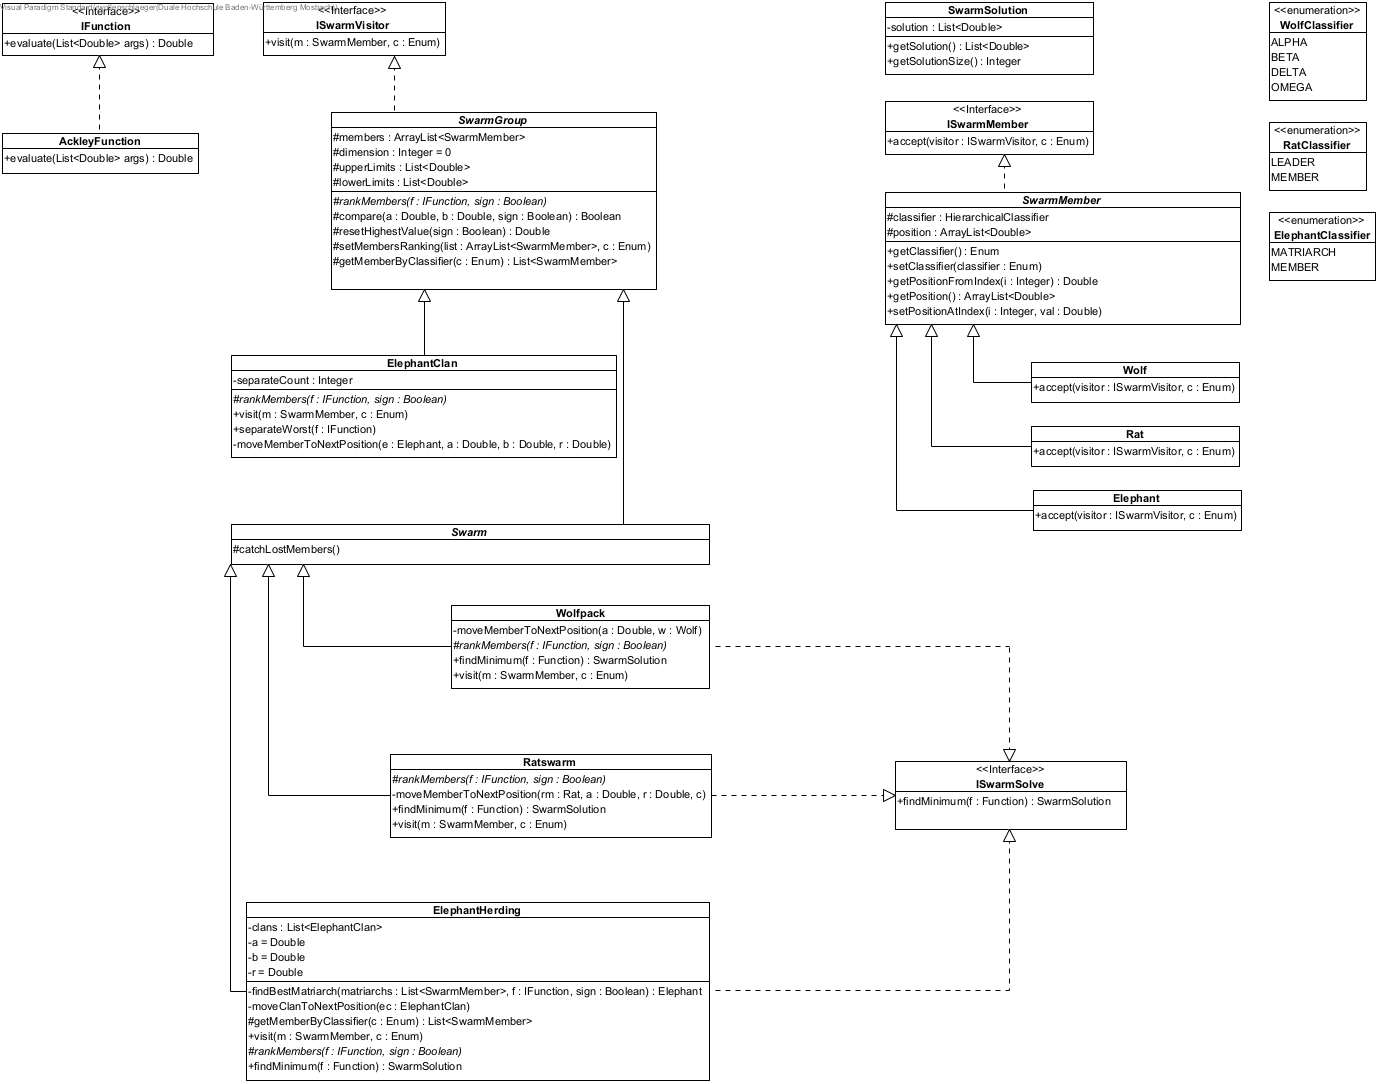
\includegraphics[width=1.0\textwidth]{../SwarmOptimization.jpg}
        \caption{UML Bibliothek Schwarmintelligenz}
        \label{uml_img}
    \end{center}
\end{figure}